\documentclass{article}
\usepackage[utf8]{inputenc}
\usepackage{minted}
\usepackage{graphicx}
\usepackage{hyperref}
\usepackage[dvipsnames]{xcolor}

\title{LoRa Mac avec Lopy4 ping pong}
\author{cmonaton }
\date{July 2019}

\begin{document}

\maketitle

\section{Introduction}

But : Envoyer des messages directement entre 2 Lopy4 en LoRa MAC c.à.d sans passer par le réseau LoRaWAN.


  \begin{figure}[H]
  \centering
  \begin{minipage}[b]{0.4\textwidth}
    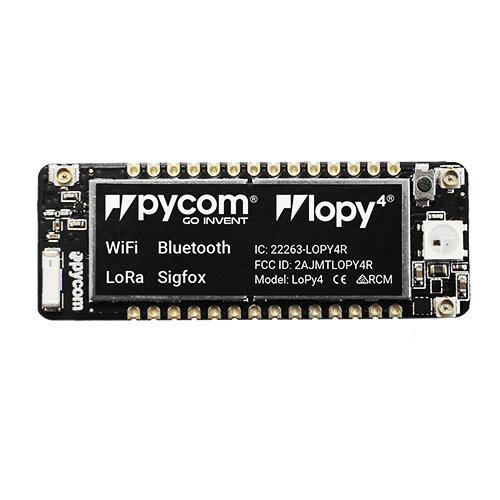
\includegraphics[keepaspectratio=true,scale=1.7]{pycom_lopy4.jpeg}
        \caption{pycom lopy 4}
  \end{minipage}
  \hfill
  \begin{minipage}[b]{0.4\textwidth}
   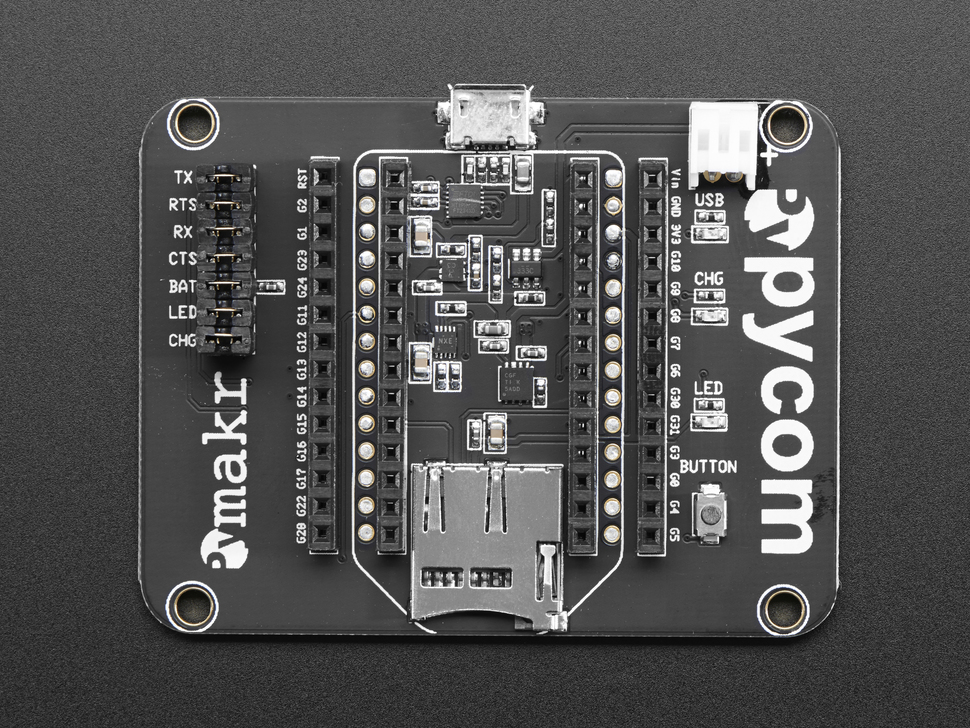
\includegraphics[keepaspectratio=true,scale=0.5]{pycom_expansion_board.jpeg}
    \caption{expansion board v3.0}
  \end{minipage}
\end{figure}

    \begin{figure}[H]
\begin{center}
\advance\leftskip-3cm
\advance\rightskip-3cm
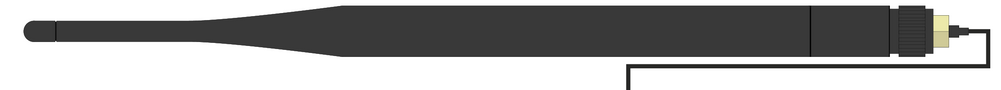
\includegraphics[keepaspectratio=true,scale=0.2]{lora_antenna.png}
\caption{antenne LoRa}
\label{visina8}
\end{center}\end{figure}


\section{Matériel}
\textcolor{red}{Branchez l'antenne LoRa avant d'alimenter la carte sinon la carte grille}

\section{Code à télécharger sur les cartes}

 Téléchargez le code à : \url{https://github.com/GitClementtest/pingpong_lopy4} \\


\subsection{Node A}
\begin{minted}{python}

from network import LoRa
import socket
import time


lora = LoRa(mode=LoRa.LORA, region=LoRa.EU868)
s = socket.socket(socket.AF_LORA, socket.SOCK_RAW)
s.setblocking(False)

while True:
    if s.recv(64) == b'Ping':
        print('Pong sending')
        s.send('Pong')
    time.sleep(2)

\end{minted}




\subsection{Node B}

\begin{minted}{python}

from network import LoRa
import socket
import time


lora = LoRa(mode=LoRa.LORA, region=LoRa.EU868)
s = socket.socket(socket.AF_LORA, socket.SOCK_RAW)
s.setblocking(False)
while True:
    data=s.recv(64)
    print(data)
    s.send('Ping')
    time.sleep(2)

\end{minted}

\section{Se connecter à la carte pour la programmer}



\subsubsection{installer Atom text editor}


Télécharger la version 1.39.0 sur \url{https://github.com/atom/atom/releases}
Téléchargez le .deb.

%\begin{minted}{bash}
%sudo add-apt-repository ppa:webupd8team/atom
%sudo apt install atom
%\end{minted}


\subsubsection{installer pymakr}
Informations complémentaires : \url{https://docs.pycom.io/pymakr/installation/atom/}

Depuis atom selon l'image installer pymakr


    \begin{figure}[H]
\begin{center}
\advance\leftskip-3cm
\advance\rightskip-3cm
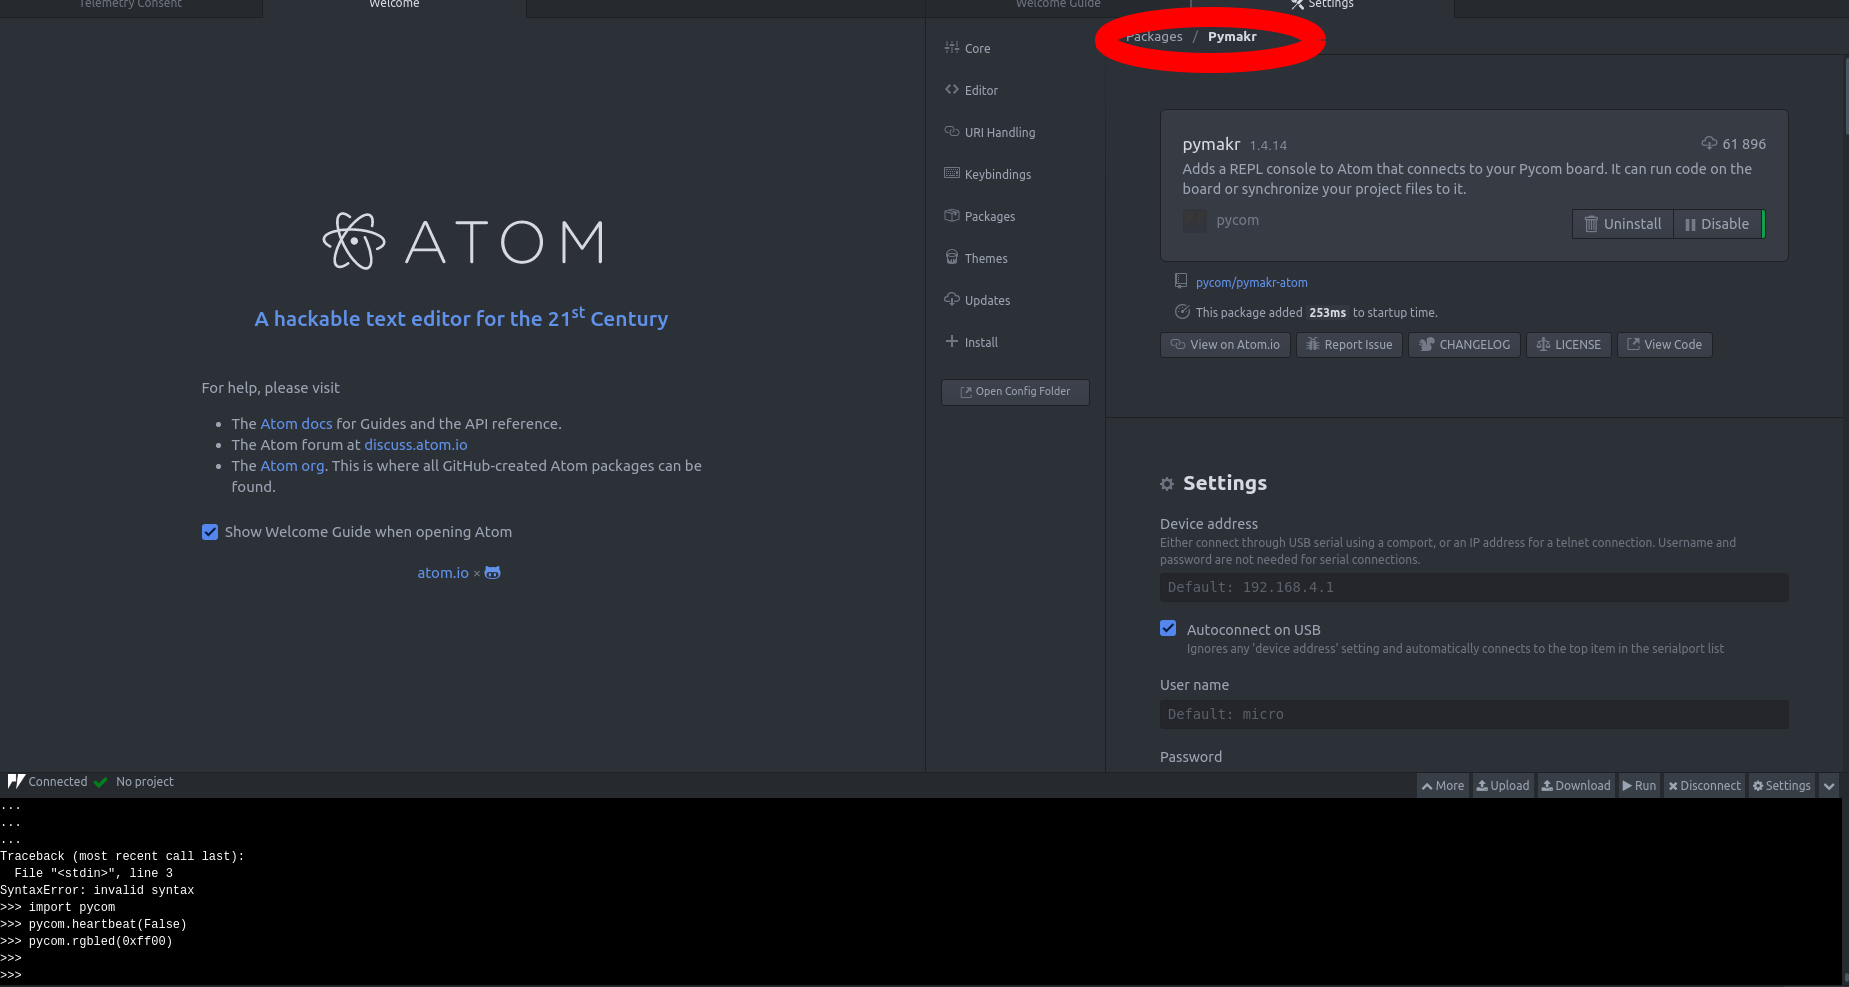
\includegraphics[keepaspectratio=true,scale=0.3]{atom.png}
\label{visina8}
\end{center}\end{figure}

Si il est impossible d'installer pymakr, essayez d'installer une version antérieure à : \url{https://github.com/atom/atom/releases},
Une alternative est aussi Visual Studio Code.


\subsubsection{Connexion à la carte}

Déterminer le port série sur lequel la carte est montée :

Après le branchement : 

\begin{minted}{bash}
dmesg | grep tty 
\end{minted}

ttyACM0 dans mon cas. Appuyez sur reset si le programme ne se lance pas.



\subsubsection{Pour ouvrir les ports ttyACM0 et ttyACM1 }

\textbf{Solution temporaire} 


\begin{minted}{bash}
sudo chmod 666 /dev/ttyACM0
\end{minted}
Il faut le entrez cette commande souvent. \\
\textbf{Solution permanente}\\

Créer un fichier dans son home

\begin{minted}{bash}
50-myusb.rules
\end{minted} 

l'éditer : 

\begin{minted}{bash}
KERNEL=="ttyACM[0-9]*",MODE="0666"
\end{minted}

Puis copiez ce fichier dans /etc/udev/rules.d/ et redémarrer votre PC.

\begin{minted}{bash}
 sudo cp 50-myusb.rules /etc/udev/rules.d
\end{minted}
C'est suffisant pour ne plus avoir à réouvrir les ports manuellement. Cependant, n'importe quel dispositif usb connecté au PC a maintenant le droit d'écriture sur le PC. \\

Pour plus de sécurité ajouter ces lignes dans ce fichier :

\begin{minted}{bash}
ACTION=="add", KERNEL=="ttyACM[0-9]*", ATTRS{idVendor}=="xxxx", 
ATTRS{idProduct}=="yyyy", MODE="0666"
\end{minted}
 
 Pour déterminer idVendor et idProduct des cartes tapez lsusb avant et après avoir connecter la carte. \\

 Dans mon cas avant et après avoir branché une carte lopy4 :
 
 \begin{figure}[H]
\begin{center}
\advance\leftskip-3cm
\advance\rightskip-3cm
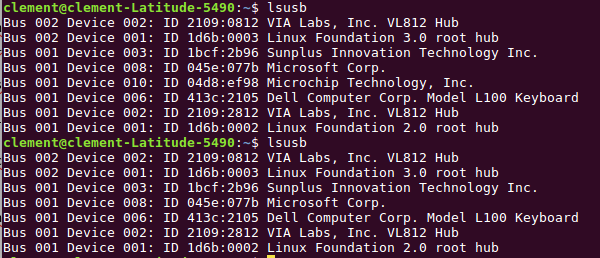
\includegraphics[keepaspectratio=true,scale=0.5]{lsusb.png}
\label{visina8}
\end{center}\end{figure}

idProduct = ef98\\
idVendor= 04d8\\

Pour ajouter d'autres appareils, copier coller ces lignes en changeant idProduct et idVendor. \\


Selon l'image utiliser la console d'Atom pour se connecter à la carte :



  \begin{figure}[H]
\begin{center}
\advance\leftskip-3cm
\advance\rightskip-3cm
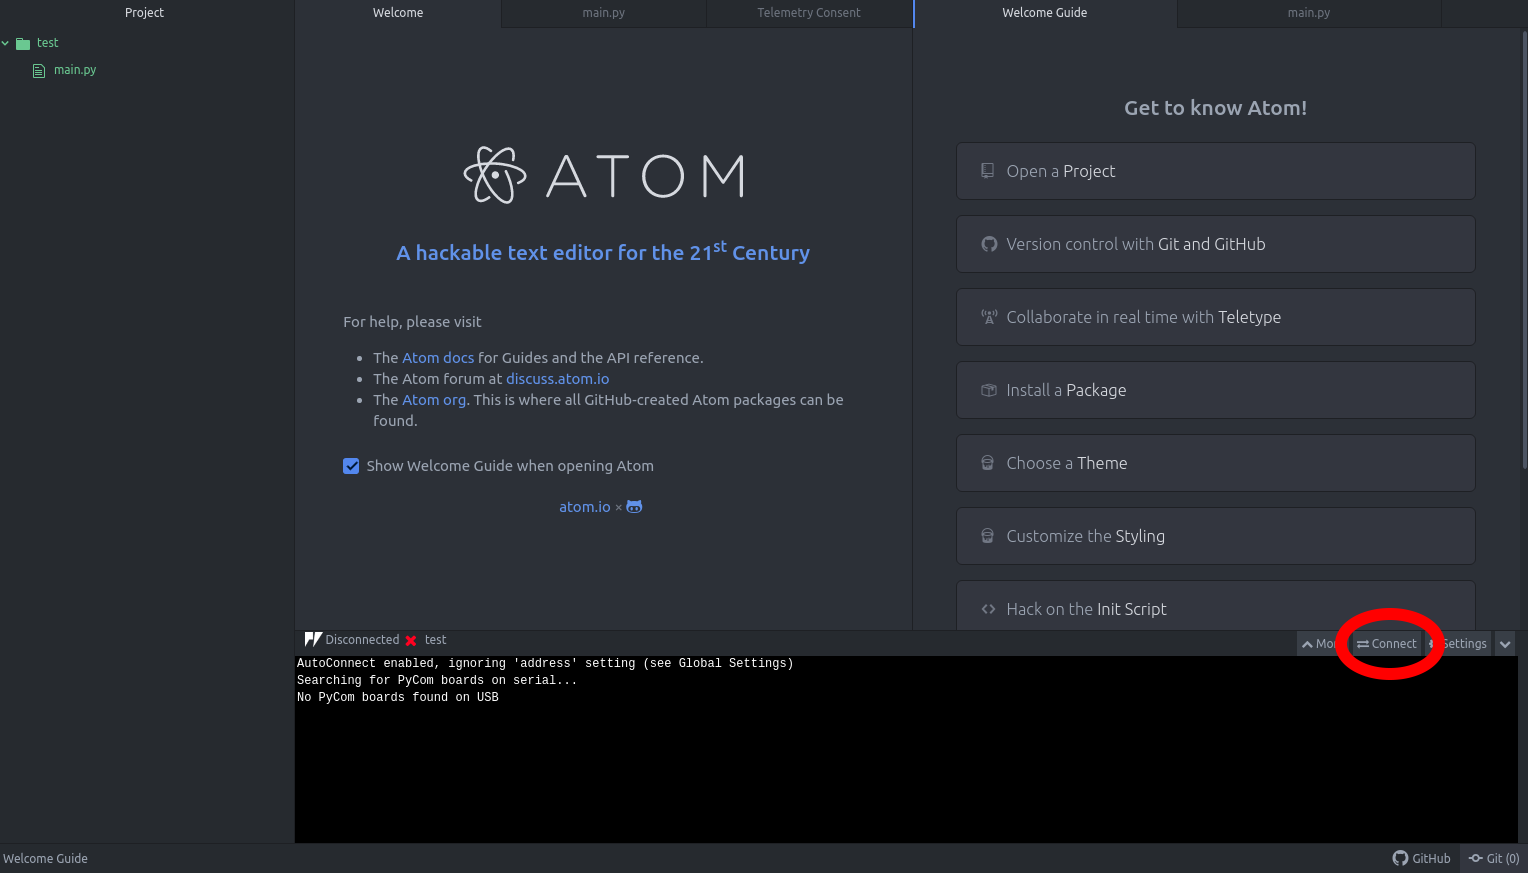
\includegraphics[keepaspectratio=true,scale=0.2]{atom_connect.png}
\label{visina8}
\end{center}\end{figure}



\subsection{Télécharger un firmware sur la carte avec Atom Pymakr}

Guide sur le site d'Atom : \url{https://docs.pycom.io/gettingstarted/programming/first-project/}\\

Créer 2 dossiers \\
Créer 1 main.py contenant le code décrit en première partie dans chaque dossier. 


\subsubsection{Connecter la carte avec Atom}
Appuyer sur le bouton connect de la console pymakr.
S'assurer que le port est ouvert est qu'aucun autre terminal série n'est ouvert sur ce port.

Dans Atom File, Open Folder pour choisir son projet puis cliquer sur Upload dans la console Pymakr pour télécharger le  code sur la carte. \\



\begin{figure}[H]
\begin{center}
\advance\leftskip-3cm
\advance\rightskip-3cm
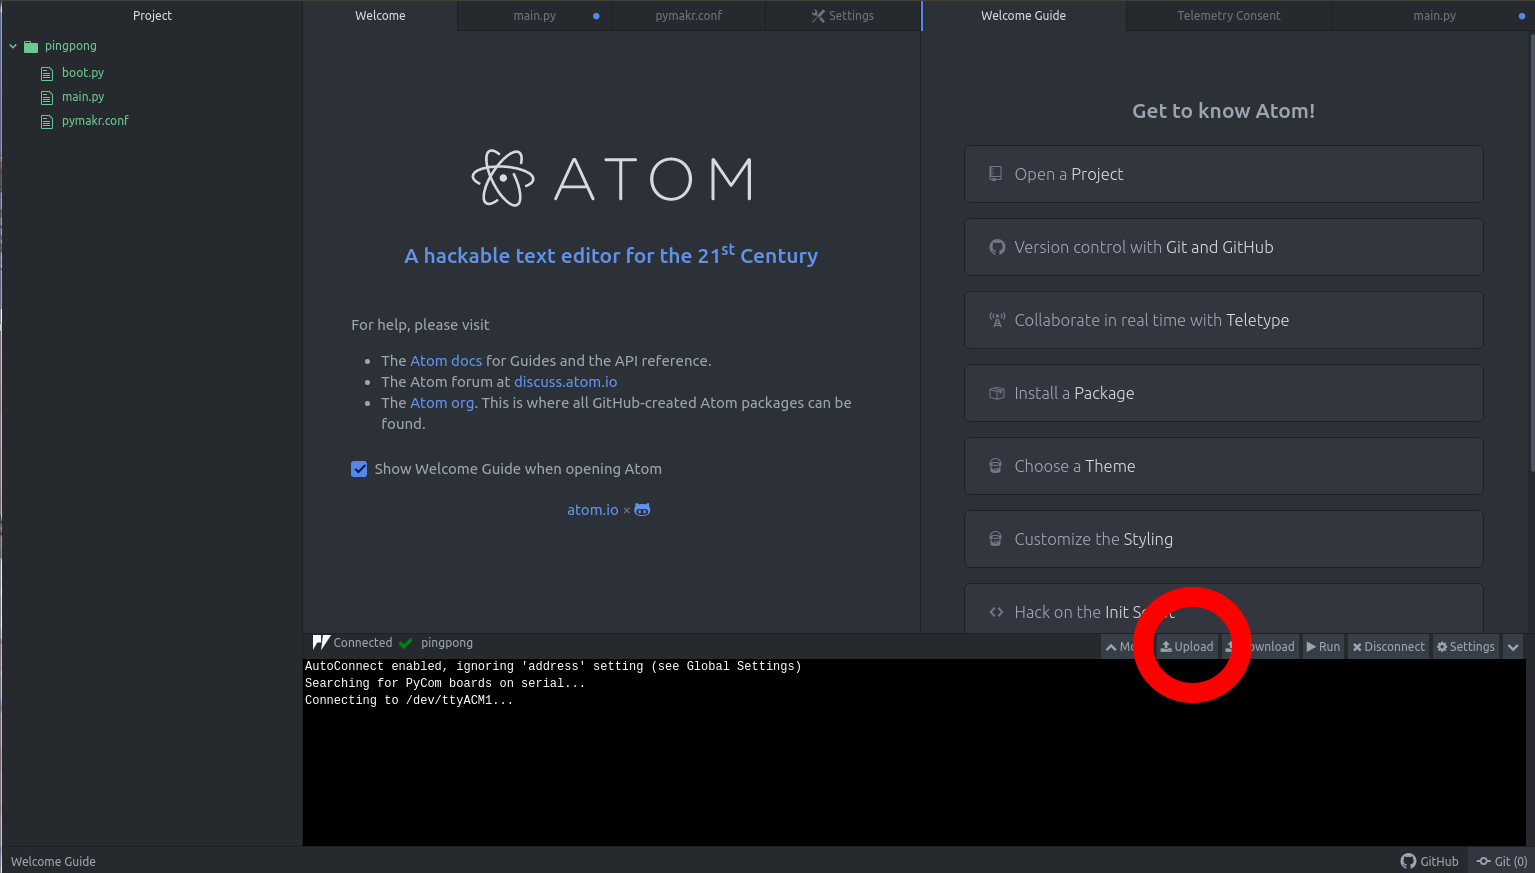
\includegraphics[keepaspectratio=true,scale=0.2]{atom_upload.png}
\label{visina8}
\end{center}\end{figure}

\textbf{Si vous copiez-collez le code attention aux identations} pour le firmware. Parfois avec des copier-coller les indentations se perdent.
Il faut coller toutes les lignes à gauche du fichier (colonne 0), sauf lorsqu'on entre dans des conditions type while, if etc. Dans ces conditions il faut 1 tabulation au début de chaque ligne.
Si ce n'est pas respecté le programme ne compile pas. \\


Après avoir téléchargé le firmware sur la carte, appuyer sur le bouton reset de la carte à côté des leds rgb pour lancer le programme.

\begin{figure}[H]
\begin{center}
\advance\leftskip-3cm
\advance\rightskip-3cm
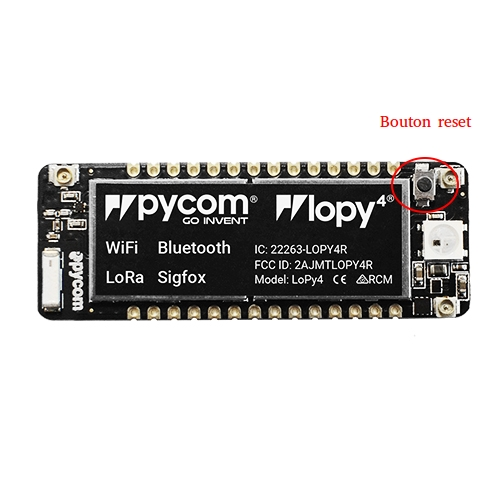
\includegraphics[keepaspectratio=true,scale=0.3]{reset.jpeg}
\label{visina8}
\end{center}\end{figure}


\subsection{Avec un terminal série type PuTTY}

PuTTY : sélectionner liaison série, choisir le bon port /dev/ttyACM0 dans mon cas, baudrate 115200.
Les cartes sont branchées sur ttyACM0 et ttyACM1 dans mon cas. 




\section{Résultat}
\begin{figure}[H]
\begin{center}
\advance\leftskip-3cm
\advance\rightskip-3cm
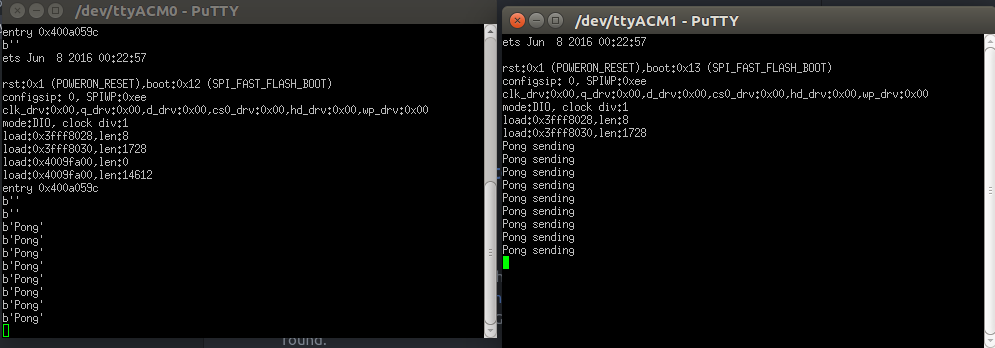
\includegraphics[keepaspectratio=true,scale=0.5]{ping_pong3.png}
\label{visina8}
\end{center}\end{figure}

\subsection{Avec minicom}
Je recommande d'utiliser minicom car on a pas besoin de réouvrir le programme à chaque fois qu'on déconnecte un appareil.

\subsubsection{Installer minicom}
\begin{minted}{bash}

sudo apt-get install minicom

\end{minted}

\subsubsection{Pour quitter minicom}


\begin{minted}{bash}

ctrl+a puis q
\end{minted}

\subsubsection{lancer minicom}
\begin{minted}{bash}
sudo minicom

\end{minted}


\subsubsection{Configurer minicom}
\begin{minted}{bash}

sudo minicom -s
\end{minted}

\section{Résultat}
\begin{figure}[H]
\begin{center}
\advance\leftskip-3cm
\advance\rightskip-3cm
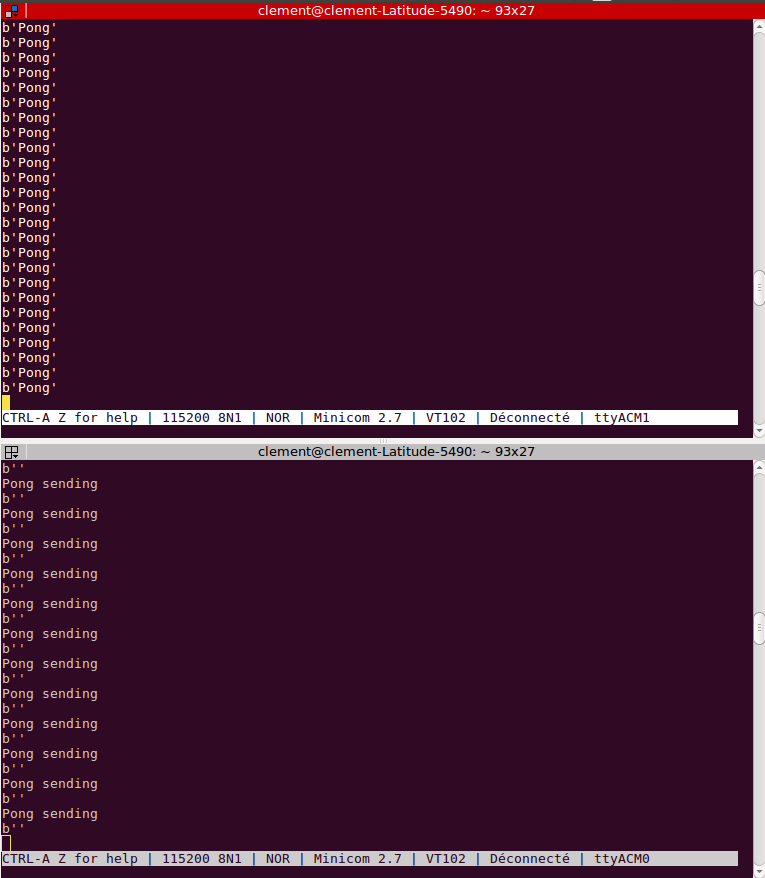
\includegraphics[keepaspectratio=true,scale=0.4]{pin_pongminicom.png}
\label{visina8}
\end{center}\end{figure}




\end{document}
